\documentclass{beamer}
\usetheme{Wrexham}  
\usepackage{graphicx}
 
\usepackage{movie15}

\begin{document}
\title{Methods for Background Subtraction in Video}
\subtitle{}
\author{Rhian Davies}

\date{\today}

\begin{frame}[plain] 
  \titlepage
\end{frame}

\begin{frame}
  \frametitle{Analysing video in Matlab}
  \begin{figure}[h]
    \centering
    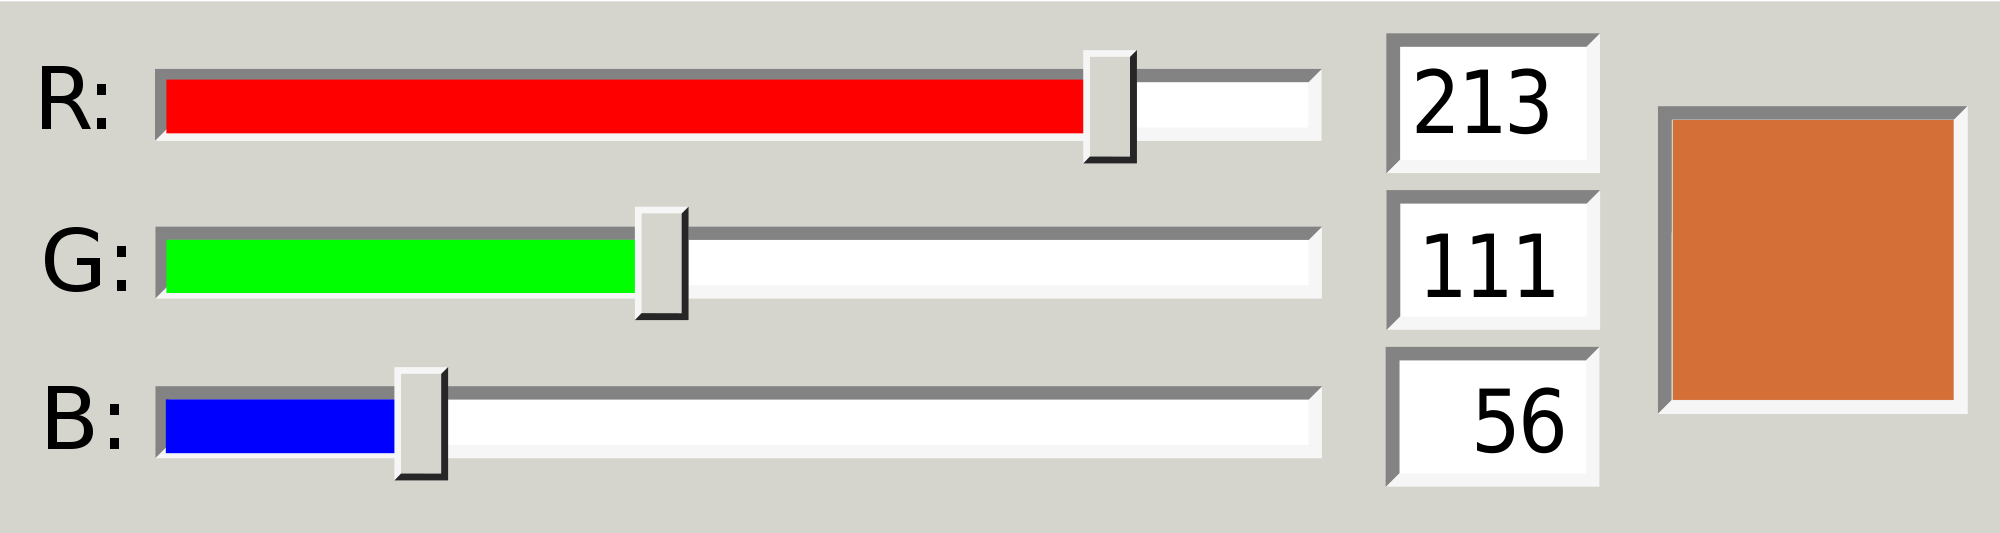
\includegraphics[height = 2.5cm]{rgbslider.png}
    %\caption{RGB slider}
  \end{figure}
\end{frame}

\begin{frame}
  \frametitle{Video test}

\begin{figure}[ht]
\includemovie[poster,text={\small(Loading Video...)}]{6cm}{4cm}{dancing_bartenders.mov}
\end{figure}

\end{frame}


%\begin{frame}
%  \frametitle{Analysing video in Matlab}
%  \begin{figure}[h]
%    \centering
%    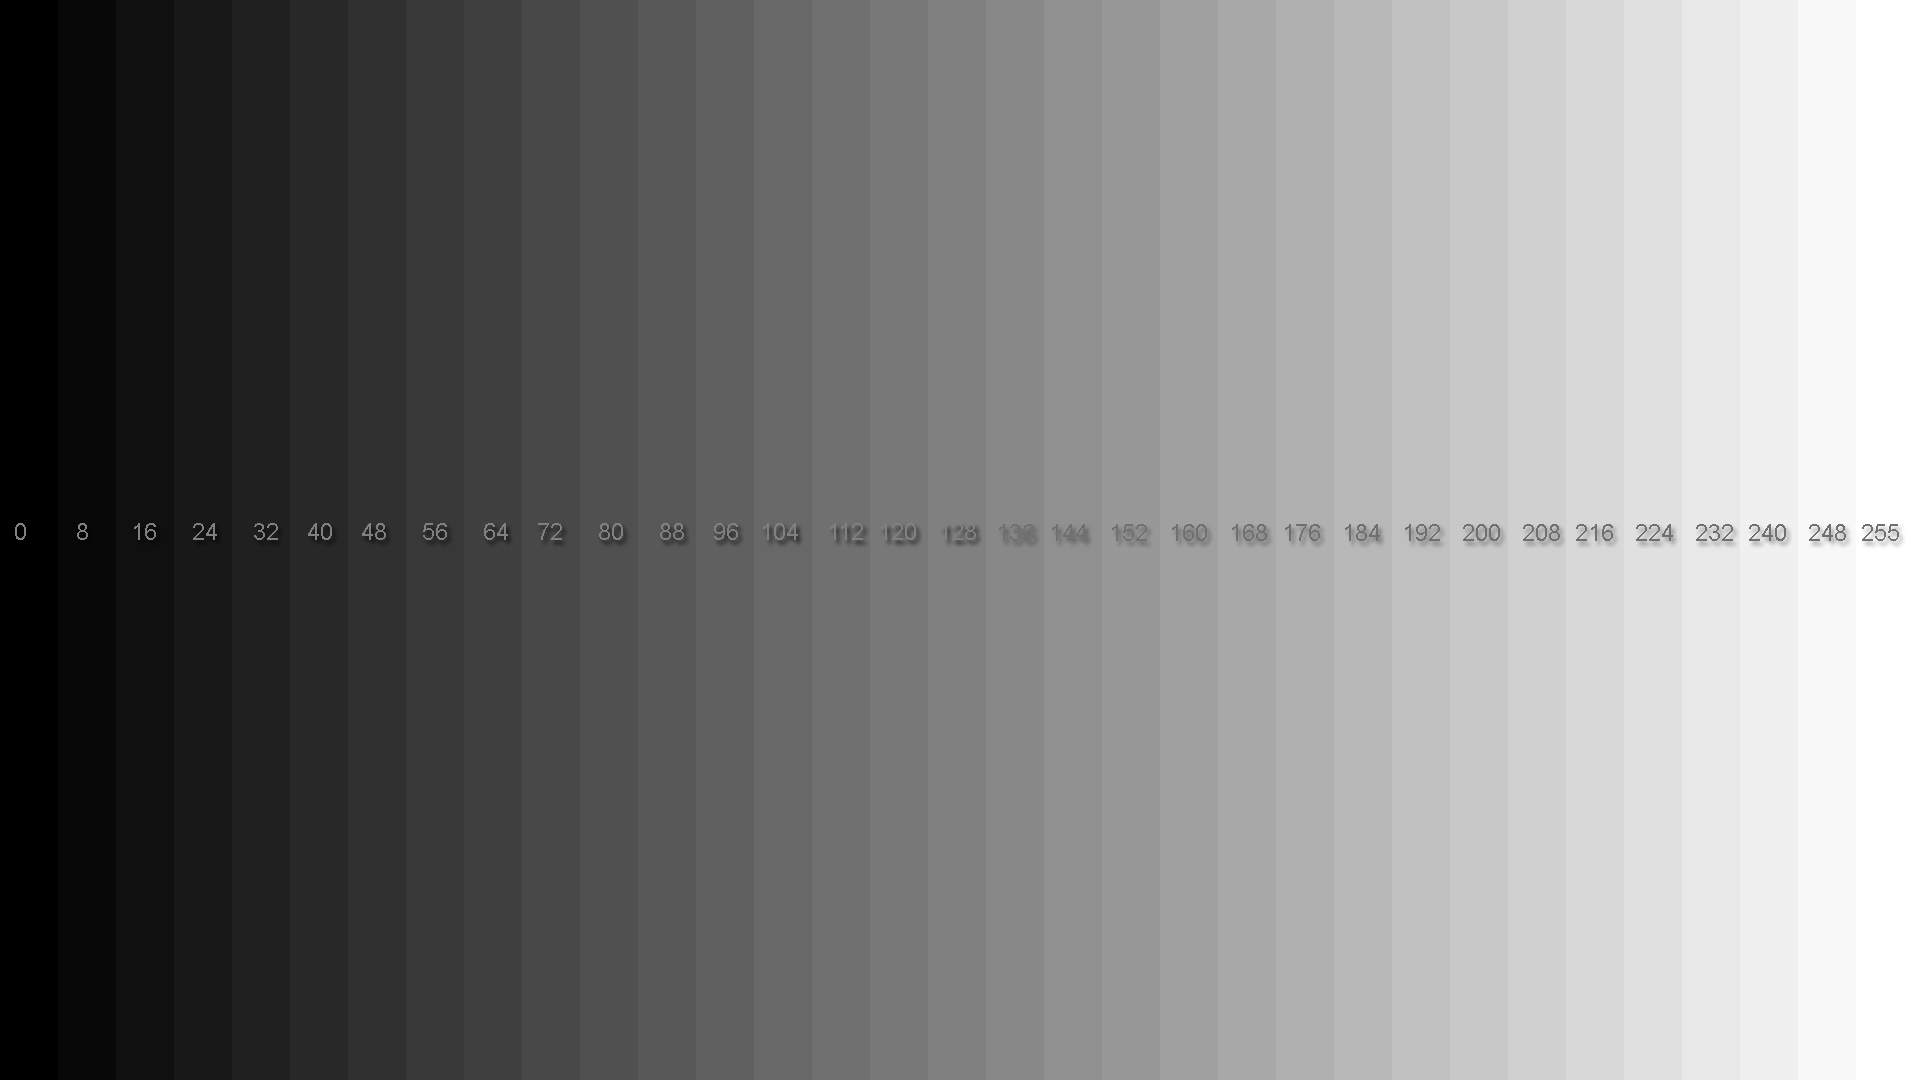
\includegraphics[height = 3cm]{grayscale.JPG}
%   % \caption{Grayscale}
%  \end{figure}
%\pause 
%\begin{figure}[h]
%  \centering
%  \[$X_t = $  \left( \begin{array}{ccc}
%54 & 106 & 69 \\
%220 & 7 & 3 \\
%6 & 45 & 101 \end{array} \right)\] 
%\end{figure}
%
%
% \begin{equation*}
%    \label{eq:3}
%X_t = [54,106,69,220,7,3,6,45,101]  \quad t= 1:T  
%  \end{equation*}
%
%\end{frame}

\begin{frame}
  \frametitle{Frame Difference}

  \begin{itemize}
  \item Assume that the first frame is the background.
  \item Accept pixel $i$ as forground if
  \end{itemize}

  \begin{equation*}
    \label{eq:1}
    |X_t[i] - X_{t-1}[i]| > \tau.
  \end{equation*}
 \pause 
  \begin{itemize}
	  \item Advantage: Computationally light, adaptive.
	  \item Disadvantage: Stationary objects can vanish
          \item Disadvantage: Interior pixels for uniformly distributed
          \item Choice of $\tau$
	\end{itemize}
 \end{frame}

\begin{frame}
  \frametitle{Approximate Median}

\[  \begin{array}{cccc}
\text{If} & X_t[i] > B[i] & \text{then} & B[i] = B[i] + 1 \\
\text{If} & X_t[i] < B[i] & \text{then} & B[i] = B[i] - 1 \end{array} \] 
\pause
  \begin{itemize}
	  \item Advantage: Seperates as a whole
          \item Advantage: Still fairly efficient 
	  \item Disadvantage: Background adapts more slowly.  
	  \item Disadvantage: Lots of ghost trails ($\tau$ dependent)
  	\end{itemize}

 \bf{Challenging real world problems require something more adaptive.}

\end{frame}

\begin{frame}
  \frametitle{Ghosts}
 
 \begin{figure}[h]
    \centering
    
\includegraphics[width=4cm ]{casper.jpg}
   % \caption{A friendly ghost}
   % \label{fig:casper}
  \end{figure}

Ghost: A set of connected points detected as motion but not corresponding to any real moving object. 
 \end{frame}
\begin{frame}
  \frametitle{Mixture of Gaussian}

  \begin{itemize}
    \item Parametric background model based on visual history.
   \item Each pixel represented by a mixture of Gaussian functions.
   \item $\mu$: educated guess of the $X_{t+1}[i]$
   \item $\sigma$: Our confidence
   \item 3-5 Gaussian components and weight them
   \end{itemize}

   \end{frame}

\begin{frame}

\begin{equation*}
      \omega_1*N(\mu_1, \sigma_1 ) + \omega_2*N(\mu_2, \sigma_2 ) + \omega_3*N(\mu_3, \sigma_3 )
   \end{equation*}

 \begin{figure}[h]
    \centering
    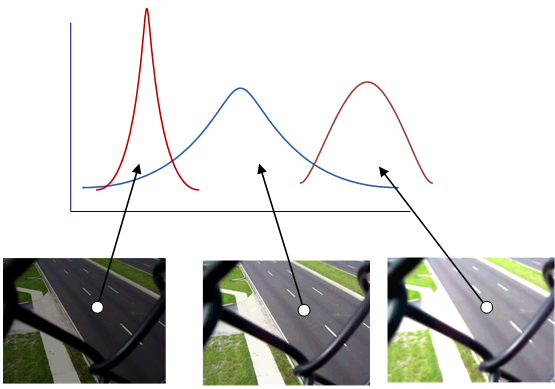
\includegraphics[width=8cm ]{mog.png}
   % \caption{A friendly ghost}
   % \label{fig:casper}
  \end{figure}
\end{frame}

\begin{frame}

  \begin{itemize}
    \item Advantage: Slow illumination changes
      \item Self corrective (parked cars)
      \item Disadvantage: Shadows
      \item Disadvantage: Physical background changes are slow.
      \item Disadvantage: Computationally heavy.
  \end{itemize}
\end{frame}

\begin{frame}
  \frametitle{Review}
  \begin{itemize}
  \item Frame difference
    \item Approximate Median
      \item Mixture of Gaussian 
  \end{itemize}

  \begin{figure}[h]
    \centering
       
\includegraphics[width=4cm ]{holygrail.jpg}%
  \end{figure}

\end{frame}

 \end{document}


